\begin{apartats}

\apartat[1,25]{1}
Troba totes les asímptotes de la funció
\[
f(x)=\frac{2x-1}{x+3} .
\]

\begin{solucio}
\textbf{Vertical}: el denominador s'anul·la en $x=-3$ i el numerador no ($-7\neq0$), i
$\lim_{x\to-3^-}f(x)=+\infty$ i $\lim_{x\to-3^+}f(x)=-\infty$: asímptota vertical
$\boxed{x=-3}$.\\
\textbf{Horitzontal}: numerador i denominador tenen el mateix grau, i
$\lim_{x\to\pm\infty}f(x)=\dfrac21=2$: asímptota horitzontal $\boxed{y=2}$.\\
Com que hi ha asímptota horitzontal, no n'hi pot haver cap d'obliqua.
\end{solucio}

\begin{nomesllarg}
\apartat{0,75}
Troba totes les asímptotes de la funció
\[
g(x)=\frac{x^2+1}{x-1} .
\]

\begin{solucio}
\textbf{Vertical}: $x=1$, perquè el denominador s'hi anul·la i el numerador val $2\neq0$.\\
\textbf{Obliqua}: el grau del numerador supera en $1$ el del denominador. Dividint,
$\dfrac{x^2+1}{x-1}=x+1+\dfrac{2}{x-1}$, i el terme que sobra tendeix a $0$: asímptota
obliqua $\boxed{y=x+1}$. No hi ha asímptota horitzontal.
\end{solucio}
\end{nomesllarg}

\apartat[1,25]{0,75}
Dibuixa la gràfica d'una funció que tingui domini $\mathbb{R}\setminus\{2\}$, asímptota
vertical $x=2$ i asímptota horitzontal $y=-1$, i escriu-ne una expressió.

\begin{solucio}
Per exemple, $f(x)=-1+\dfrac{1}{x-2}$: el domini és $\mathbb{R}\setminus\{2\}$, en $x=2$ els
límits laterals són $\mp\infty$ i $\lim_{x\to\pm\infty}f(x)=-1$.
\begin{center}
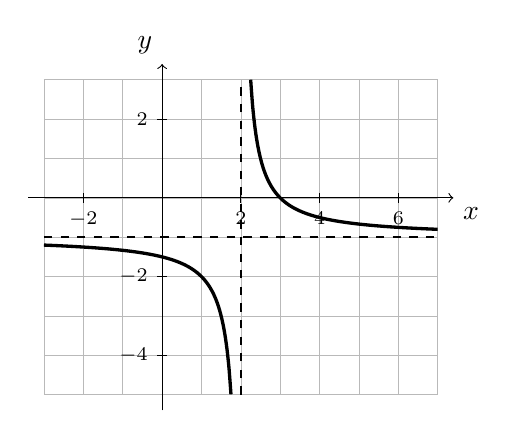
\begin{tikzpicture}[x=0.5cm,y=0.5cm]
  \draw[gray!55,very thin,step=1] (-3,-5) grid (7,3);
  \draw[->] (-3.4,0) -- (7.4,0) node[below right] {$x$};
  \draw[->] (0,-5.4) -- (0,3.4) node[above left] {$y$};
  \foreach \i in {-2,2,4,6} \draw (\i,0.12) -- (\i,-0.12) node[below,font=\scriptsize] {$\i$};
  \foreach \j in {-4,-2,2} \draw (0.12,\j) -- (-0.12,\j) node[left,font=\scriptsize] {$\j$};
  \draw[dashed,thick] (2,-5) -- (2,3);
  \draw[dashed,thick] (-3,-1) -- (7,-1);
  \begin{scope}
    \clip (-3,-5) rectangle (7,3);
    \draw[\colorgrafica,very thick,domain=-3:1.75,samples=100,smooth] plot (\x,{-1+1/(\x-2)});
    \draw[\colorgrafica,very thick,domain=2.25:7,samples=100,smooth] plot (\x,{-1+1/(\x-2)});
  \end{scope}
\end{tikzpicture}
\end{center}
Qualsevol altra funció amb aquestes asímptotes també val.
\end{solucio}

\end{apartats}
